\begin{figure}[h!]
	\centering
	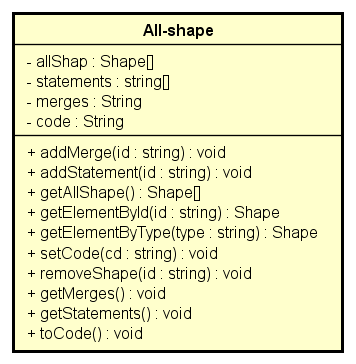
\includegraphics[scale=0.8]{res/sections/SpecificaFrontEnd/Services/Disegnetti/all-shape.png}
	\caption{Diagramma della classe All-shape}
\end{figure}

\begin{itemize}
	\item \textbf{Descrizione:}\\
	Servizio che contiene tutte le shape inserite nell'editor permettendone l'aggiunta e la rimozione, e ii metodi per trasformare i diagrammi in codice
	\item \textbf{Utilizzo:}\\
	É possibile aggiungere ed eliminare le shape inserite nel diagramma, necessarie per la creazione del codice.
	
	\item \textbf{Attributi:}
		\begin{itemize}
			\item \emph{-allShap: Shape[]}\\
			Rappresenta l'array di shapes
			\item \emph{-statements: string[]}\\
			Rappresenta lo stato delle shapes
			\item \emph{-merges: string}\\
			Ritorna il risultato delle shapes mergiate
			\item \emph{-code: string}\\
			Contiene il codice generato dal metodo
		\end{itemize}
	\item \textbf{Metodi:}
		\begin{itemize}
			\item \emph{+addMerge(id: string)}\\
    		Aggiunge il codice corrente al progetto\\
    		\textbf{Parametri:}
    		\begin{itemize}
    			\item \emph{id: string}\\
    			Progetto
    		\end{itemize}
    		\item \emph{+addStatement(id: string)}\\
    		Aggiunge lo statement alla decisione\\
    		\textbf{Parametri:}
    		\begin{itemize}
    			\item \emph{id: string}\\
    			Statement da aggiungere
    		\end{itemize}
    		\item \emph{+getAllShape()}\\
    		Ritorna tutte le shapes
    		\item \emph{+getElementById(id: string)}\\
    		Ritorna il riferimento alla shape selezionata\\
    		\textbf{Parametri:}
    		\begin{itemize}
    			\item \emph{id: string}\\
    			Shape selezionata
    		\end{itemize}
    		\item \emph{+getElementByType(type: string)}\\
    		Ritorna il riferimento alla shape selezionata\\
    		\textbf{Parametri:}
    		\begin{itemize}
    			\item \emph{type: string}\\
    			Shape eselzionata
    		\end{itemize}
    		\item \emph{+setCode(cd: string)}\\
    		Setta la variabile code con il nuovo valore\\
    		\textbf{Parametri:}
    		\begin{itemize}
    			\item \emph{cd: string}\\
    			Nuovo valore
    		\end{itemize}
    		\item \emph{+removeShape(id: string)}\\
    		Rimuove la shape selezionata\\
    		\textbf{Parametri:}
    		\begin{itemize}
    			\item \emph{id: string}\\
    			Shape da rimuovere
    		\end{itemize}
    		\item \emph{+getMerges()}\\
    		Ritorna l'attributo merges
    		\item \emph{+getStatements()}\\
    		Ritorna l'attributo statements
    		\item \emph{+toCode()}\\
    		Converte le shape in codice
		\end{itemize}
\end{itemize}